\documentclass[../main.tex]{subfiles}
\graphicspath{{\subfix{../IMAGES/}}}

\begin{document}
\localtableofcontents

\subsection{Introduction}

Global GHG emissions : $57GT$ $CO_{2-eq}$. Energy and methane leaks have an important port of the emissions. Primary energy consumption is around $172000 TWh$. \\
Some key indicators to understand the state of the world : extreme poverty, GDP per capita, population, child mortality, fertility rate, life expectancy, hunger, education, access to water and sanitation, \textbf{energy access}, \textbf{energy use}, \textbf{$CO_2$ emissions}.\\

\textbf{Production based emissions} are computed within country boundaries, without accounting how goods are traded across the world.\\
\textbf{Consumption based emissions } account for trade of goods. Imported goods need to add $CO_2$ emissions emitted in the production of these goods. Exported goods need to subtract $CO_2$ emissions. \\
Switzerland : annual emission from 4.2 tons to 12 tons of $CO_2$ per capita if consumption based.\\

Why is Sweden good at lowering both? Growing carbon tax, increasing renewable energy sources and EV, improving energy efficiency, promoting sustainable transportation, encouraging sustainable consumption and production.\\

\quad \underline{Major energy units :}\\
1l of oil $\simeq$ 1$m^3$ of NG $\simeq$ 10 kWh. 1l of gasoline $\simeq 9kWh$.\\
1 ton of oil equivalent (Toe) = 41.868TJ\\
Barrel of oil equivalent (BOE) = 6.1GJ\\
1 british thermal unit (BTU) = 1055.06J\\

\quad \underline{Orders of magnitude :}\\
\begin{itemize}
    \item Nuclear PP : $0.4-1.6GW$ per unit, $c_p = 80-90\%$
    \item Coal-fired PP : $200MW-1GW$ per unit, $c_p = 70-90\%$
    \item Hydroelectric PP : $0.5-22.5GW$, $c_p = 30-90\%$
    \item Wind PP : $200MW-20GW$ onshore, $200MW-1.2GW$ offshore, $c_p = 25-55\%$
    \item Solar PP : $200MW-5GW$, $c_p = 12-30\%$
    \item Geothermal PP : $10-250MW$ per unit, $c_p = 65-75\%$
    \item Daily world oil demand : $100M$ barrels (160TWh)
    \item Annual household electricity demand : $3000 kWh$
    \item Total USA energy consumption annually : $26 000TWh$
    \item Total world NG consumption annually : $40 000TWh$
    \item Total world electricity production annually : $28600 TWh$
    \item Total world energy consumption annually : $160 000 TWh$
\end{itemize}

Average efficiency for electricity PP : coal is around $31.7\%$, petroleum is around $31\%$, NG is around $44.2\%$, nuclear is around $32.6\%$. Up to $62\%$ for gas combined cycled powerplants.\\
Process efficiency : EV is around $70-85\%$, ICE is around $16-25\%$, wind turbine is around $35-45\%$ and geothermal plant is around $10-20\%$.\\

\textbf{Primary energy} is an energy form found in nature that has not been subjected to any human engineered conversion process. \\
\textbf{Total Primary energy supply (TPES)} is the sum of production and imports subtracting exports and storage changes.\\
\textbf{Secondary energy sources are energy carriers } derived from the transformation of primary energy sources.\\

\quad \underline{How to count primary energy ?}\\
\begin{itemize}
    \item Direct equivalent method : distinguishes between combustion and non-combustion electricity combustion. Electricity generated from all non-combustible energy sources is primary energy.
    \item Physical energy content method : distinguishes between thermal and non-thermal sources of electricity (incl. nuclear). Thermal energy generated from nuclear, geothermal, solar and fossil is primary energy.
    \item Substitution method : computes the primary energy content of non-combustible sources by determining how much fossil fuel would be necessary to generate the same amount of electricity. It applies to wind, solar, hydro, nuclear and all non-combustible method by multiplying by 2.5 the kWh electrical. Assumes $40\%$ efficiency.
\end{itemize}

\subsection{CO2 equivalent emissions and GW}
Annually, over $37bT$ $CO_2$-eq. \\
Cement represent $2.3GT$ of $CO_2$/year. Iron and steel release $2.6 GT$ of $CO_2$/year. $CO_2$ from aviation globally was $2.5\%$ in 2020.\\

Fossil fuels burnings have an impact on health; they are the major reason for global warming.\\
In average, temperature increased more than $1.5^\circ C$ from 1950. Slope tends to accelerate. \\

Impact of GW : sea level rising (0.3-0-6m for a low-emission scenario), costal erosion, population migration, food security risks. \\

Oil is mostly used for road ($49\%$) and then petrochemicals. Biofuel corresponds to $2\%$ of the world oil production. Biomass needs large areas ($\simeq 5TWh/1000km^2$)!\\
The share of renewable energy is increasing in most region. 

In 2023, 508GW of hydro and biomass installed corresponding to 110 nuclear PP running continuously. Likely in 2024, addition of 600GW of solar and 150GW of wind. In 2024, $29\%$ of electricity from wind and solar. \\
A rule of thumb is that emission will still increase by $0.5\%$ in 2024. \\

\quad \underline{Levelised Cost of Electricity (LCOE) :}\\
$LCOE = \frac{\text{CAPEX+total OPEX}}{\text{total electricity production}} $.\\

Nuclear fission contribute to $CO_2$ reduction. Currently, 52 nuclear reactors in construction. Strong variation in the LCOE : from 4cts/kWh (Korea) to 13cts/kWh (UK). Nuclear will be a partial option for loss $CO_2$ emission. \\
On-shore EU wind cost decreases ($1.3M$€/MW) with an average LCOE at 4cts/kWh. In Chine, windturbine are at $0.4$€/W. In 2023, c-Si PV module were down to 10cts/W. New large solar and large wind parks can offer electricity down to 1.3 to 3cts/kWh in windy and sunny countries. Investments are small sized. New renewables are better than coal gas or nuclear in terms of direct LCOE in most of the regions of the world. \\

Carbon capture and storage (CSS) is the separation and capture of $CO_2$ from the emissions of industrial processes and storage of the $CO_2$ in deep underground geologic formations (placement of $CO_2$ into subsurface formation). First large scale installation will have a large investment costs : $\simeq 100$€/ton.\\
Direct air capture (DAC) will be costly for several decades ($\simeq 100$€/ton in 2050, right now it is more at 500€/ton as it needs $250kWh/ton$ of electricity).\\

Biological carbon sequestration : plants absorb $CO_2$ from the atmosphere and store some as aboveground and belowground biomass. \\

Better insulated and designed house can save up to $2/3$ of energy. Better control of hidden consumptions. Energy saving bulb, appliances. Use electricity instead of fuels to power engines (gain a factor 3), use electricity and heat pump (gain a factor 3 to 5). A well designed and insulated house could reach $50kWh/m^2$. \\
Build with materials that embed $CO_2$ (e.g. wood). \\
Sources of GHG emissions : emissions of $N_2O$ (drainage of organic soil, irrigation practices, synthetic fertilizer), livestock ($CH_4$, $10-15\%$ emissions of $CO_2$ worldwide), management manure from livestock. \\

How much does the energy transition cost? IRENA gives high estimates : investments costs up to $3.8$ Trillions/year. Strong improvement in components costs including battery costs will make the bill lower. China will fight against Oil and gas producer and try to export its technologies. \\

\subsection{Energy transition}
Germany increased its share of renewable in electricity. In 2024 : $17\%$ from wind and $11\%$ from solar in Europe. Pakistan was the 4th largest country installing in PV installation.\\

For Switzerland : 37GW of PV by 2050. Now 45 TWh of new renewables in government plan for 2045.\\

What should happen globally? Develop massively wind and solar : maintain nuclear base to facilitate transition, keep and optimize fossil fuel assets, capitalize on electrochemical storage. Sufficiency : rethink consumption; accept less in critical period. Energy efficiency : switch to electrical, track losses. Agriculture : sequestration through biomass and soils. \\

\subsection{Supporting technologies and sustainability}
\quad \underline{PHS :}\\
Potential energy stored in reservoir above a turbine. Around $160GW$ capacity in 2020. Around $1000$€/kW.\\

\quad \underline{Batteries :}\\
Same learning curve as wind and solar. Today : $100-120$€/kWh for a battery pack. Battery cell can be around $47$€/kWh with 4000-5000 cycles : $1cts/kWh$.\\

\quad \underline{Thermal energy (TES) :}\\
Use heat (solar) or excess electricity. Heat up to $95^\circ C$ for winter district heating. Announced at $4cts/kWh$.\\

\quad \underline{P2G :}\\
Electrolysis of hydrogen will likely be the most meaningful route, thanks to ultra-low cost renewable and electrolyzer. Market entrance for alternative route with Ammonia. Later transport and use green Ammonia. Easier to transport than $H_2$ by boat. Still better to go all electric.\\

\quad \underline{Heat pump :}\\
Need to reach 60 millions of heat pumps by 2030. In CH more than 43 000 heat pumps in 2023.\\

\quad \underline{Transport :}\\
Road passenger emit the most. Electric car deployment has accelerated with news sales in the $20\%$ range of the full parc for around 17 millions cars. \\

\subsubsection{Sustainability}
At the scale of the energy transition, the limitation in materials is a myth. \\
For metals, mining, good practice are required. \\
With $>50Gt CO_2$, including $38Gt$ direct $CO_2$ annually we are changing the world. All oil/gas producers want to exploit as much as they can their reserves. Only realistic scenarios to decarbonize the world are based on a strong increase in electrification.\\
Sufficient and less absurd consumption will help make transition more quickly. Green economy works. Agriculture needs to reduce emission. 


\subsection{Decoupling}
Decoupling harbours the possibility to sustain economic growth while shrinking environmental impacts. Absolute decoupling is much easier when underlying activity causing the impact grows more slowly.\\

\begin{center}
    Impact = Activity x Impact/Activity
\end{center}
Resource intensity is defined as the Impact/Activity. Intensity is the inverse. \\
Efficiency is measured by how much service/activity is obtained with a given quantity of resource. \\
\textbf{Relative decoupling} : impact grows but at a smaller rate than activity, resource intensity decreases but less than growth in activity.\\
\textbf{Absolute decoupling} : impact decreases despite the growth in activity, resource intensity decreases more than growth in activity.\\

\begin{center}
    I = GDP x I/GDP\\
    $g_I = g_{GDP} + g_{I/GDP}$
\end{center}
With I the environmental impact, I/GDP the environmental or resource intensity of the economy.\\
Assume $g_{GDP} >0$, relative decoupling : $0<g_I<g_{GDP}$, absolute decoupling : $g_I < 0$.\\

\subsubsection{IPAT and Kaya decomposition}
\begin{center}
    Impact = Population x Affluence x Technology (I = Pop x GDP/Pop x I/GDP)
\end{center}
Calling I/GDP technology is a bit of a stretch. GDP : what is produced, services, industrial goods....
The Kaya decomposition ; $CO_2 emissions = Pop\times \frac{GDP}{Pop} \times \frac{E}{GDP} \times \frac{CO_2}{E}$ or $\% CO_2 = \% Pop + \% (\frac{GDP}{Pop}) + \% (\frac{Energy}{GDP}) + \%(\frac{CO_2}{Energy})$.\\
The IPAT framework can be used to compare countries. \\
Finer decomposition of $CO_2$ : $CO_2 = GDP \times \sum_j \frac{Prod_j}{GDP} \times \frac{E_j}{Prod_j} \times \frac{CO_{2j}}{E_j}$.\\

\subsubsection{Efficiency, substitution, sufficiency}
Reduce activity : avoir energy use and aim for sufficiency in activity. Reduce Energy/Activity : improve energy efficiency. Reduce $CO_2$/Energy : shift to or substitute by lower emissions energy.\\

Sufficiency is when you renounce some good or service not because you do not like it, cannot afford it, are not allowed to buy it or do not have the time for it, but only because it is harmful for the environment.

\subsubsection{Limitations of IPAT}
Diversity is hidden behind aggregates. The P,A and T component are seen as levers when one tries to influence them with a view to lowering I. They affect one another.\\

\subsubsection{Rebound effect}
Efficiency gains leads to an increase in consumption. \\

Conditions for sustainable decoupling : avoid shifting polluting activities to lower-income countries, handle the environmental impacts of the green alternatives (land use of agrofuels, minerals for electric machines and renewables, social political and environmental risks of nuclear and large hydropower generation), tackle the rebound effect (direct rebound : increased use of cheaper service, indirect rebound : damaging use of money saved), make sure that there is a substitution not just addition, do not forget limits (recycling limits), technical progress should improve rather than worsen the situation.\\

\subsection{Energy economics}
Fossil energy companies have valued on the stock market the equivalent of $762GtCO_2$ of exploited and exploitable reserves (other owner own 3 times more). Budget compatible with $+1.5^\circ C$ is $420GtCO_2$. Several factors make it more expensive to transition away from fossil : recent investments in the fossil energy extraction infrastructure, recent investments in fossil energy using infrastructure, long-term delivery contracts, businesses and manpower invested in activities related to fossil energy. \\

Investor invests sum $S_0$ now, his investment is worth $S_n$ after n year : $S_n = S_0(1+r^*)^n$, $r^*$ the \textbf{rate of return} on this investment. Consider an alternative investment promising rate of interest i : $S_n = S_0(1+i)^n$. \textbf{Arbitrage} $r=i+p$ where p is an interest premium for differences in risk and liquidity.\\

Investor expect payments of $D_1$ after 1 year, $D_2$ after 2 years, ..., $D_n$ after n years. The willingness to pay can be estimated by : $S_0 = \sum_{k=1}^n \frac{D_k}{(1+r)^k}$ : \textbf{Discounted Cash Flow (DCF)}.\\
If the investor had to invest $I_0$ for these payments, one can define the \textbf{net present value (NPV)} : $NPV = -I_0+DCF$.\\
For all regular investments, $\exists r^* $s.t. $NPV=0$, this is the internal return rate. The larger r, the smaller the NPV. There also exists a number of years $n^*$ of positive incomes that makes the NPV=0 : \textbf{payback period}. Stranded assets are assets that stop generating income before $n^*$.\\

The price of shares depends on buyers' willingness to pay for them, which is high as long as buyers anticipate profits, buyers' trust that they can sell their shares at a good price when they want. \warning It all depends on expectations. \\
The hurdle rate is the required rate of return for this type of investment. $I(r)$ is the amount that can be invested with IRR (internal rate of return) greater than hurdle rate. Anything that lowers the hurdle rate/raises the IRR triggers more investment. \\

\subsubsection{LCOE}
Initial investment cost : $C_0$ (CAPEX), recurring annual op. cost (OPEX) : $C_t$, generating quantity of electricity/year over n years : $Q_t$, scrap value at EoL : $V_n$, p is the unit price at which electricity can be sold (LCOE), capacity factor : $c_f$. \\
$NPV = -C_0 + \sum_k \frac{pQ_k-C_k}{(1+r)^k} + \frac{V_n}{(1+r)^n}$. \begin{equation}
    LCOE = \frac{C_0 + \sum_t \frac{C_t}{(1+r)^t - \frac{V_n}{(1+r)^n}}}{8760\times \sum_t \frac{c_f}{(1+r)^t}} = \frac{n CAPEX\times CRF+OPEX}{8760 \times Capacity\: factor}
\end{equation}

$CRF = \frac{r(1+r)^n}{(1+r)^n-1}$ is the \textbf{capital recovery factor}.

\subsection{Energy needs}

\begin{table}[hbt!]
    \centering
    \begin{tabular}{c|c|c|c|c}
         & Being & Having & Doing & Interacting \\ \hline
       Subsistence  & &&&\\
       Protection &&&&\\
       Affection &&&&\\
       Understanding &&&&\\
       Participating &&&&\\
       Idleness &&&&\\
       Creation &&&&\\
       Identify &&&&\\
       Freedom &&&&\\
    \end{tabular}
    \caption{Matrix of needs and satisfiers.}
\end{table}

Human needs can also be defined by the theory of human need (Doyal \& Gough 1991).\\

Biophysical resource use encompasses planetary processes and natural resources. Provisioning systems include physical (infrastructure, technology, ...) and social (governments, communities, ...). Social outcomes include need satisfiers (food, clean water, ...) and human well-being (health, life satisfaction, ...).\\

Sufficiency is a desirable organizing principle of society opposed to today's dominant efficiency. It is a set of measures and daily practices that avoid demand of energy, materials, land and water while delivering human wellbeing for all within planetary boundaries.

Decent Living Standards (DLS) : essential requirements for wellbeing. \\

The gini index expresses the level of inequality (0 if no inequality).\\

\subsection{Integrative analysis of the energy transition}
What is a transition? Multi-phase perspective : predevelopment, take-off, acceleration, stabilization.\\
Energy transition is a complex issue encompassing technical, ecological and social domains. Technological, institutional and social "lock-in". 

\begin{figure}[hbt!]
    \centering
    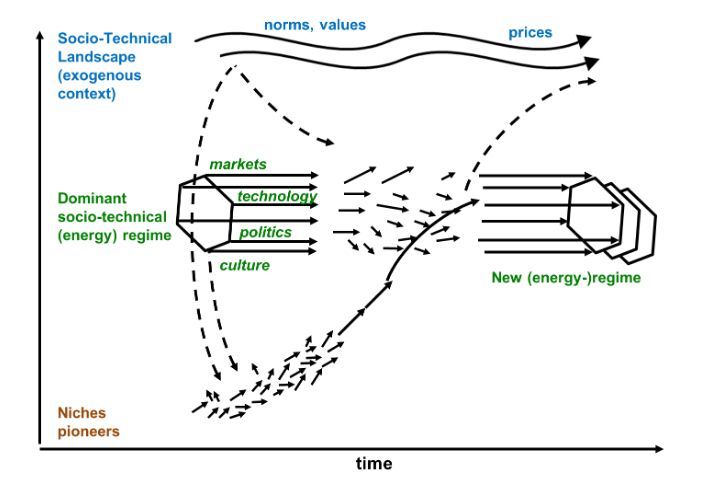
\includegraphics[width=0.5\linewidth]{IMAGES/NRJ_supply/Screenshot from 2025-04-16 08-37-13.png}
\end{figure}

Regimes : locked-in, path-dependent configurations developed in response to the needs of the past. Landscape : contextual factors that stabilize/put pressure on regimes. Niches : alternatives to dominant practices, with potential to regime change. \\

\begin{figure}[hbt!]
    \centering
    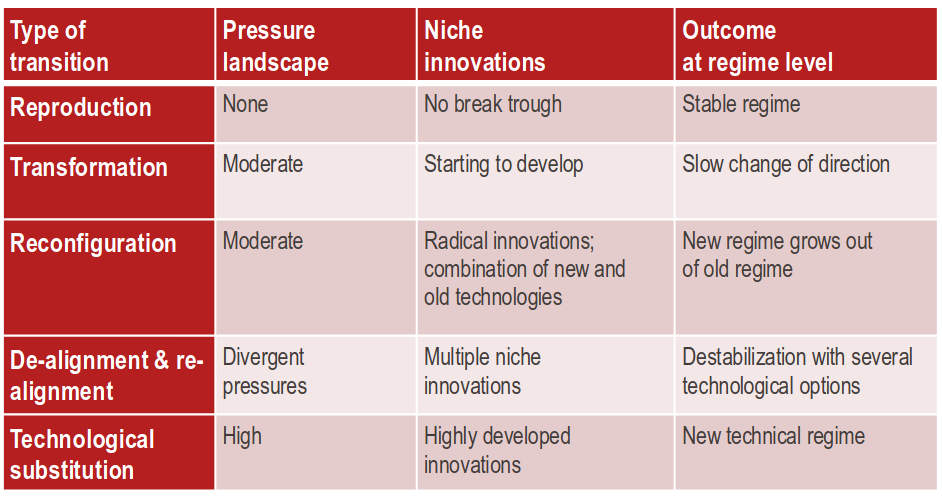
\includegraphics[width=0.5\linewidth]{IMAGES/NRJ_supply/Screenshot from 2025-04-16 08-41-48.png}
\end{figure}

How to analyze a transition? System knowledge : what are the relevant processes/flows/actors/institutions/regulatory mechanisms of the system? Goal knowledge : which goals do we define for sustainability? Transformation knowledge : what are triggers and drivers/barriers for change?\\

Individual visionary people are key drivers of the transition. Co-evolution of social-ecological-technical systems (SETs) : visionary and institutional milestones precede physical ones. External "events" can fuel the transition.\\

SDG targets number 7 : affordable and clean energy. 7.1 : ensure universal access to affordable, reliable and modern energy services. 7.2 : Increase substantially the share of renewable energy. 7.3 : double the global rate of improvement in energy efficiency. They are pretty vague.\\

\textbf{Tipping point :} point of threshold at which small quantitative changes in the system triggers a non-linear change process that is driven by system-internal feedback mechanisms and inevitably leads to a qualitatively different state of the system, which is often irreversible.\\
A cascade change is triggered when $25\%$ of a population embraces an idea. \\
Three phases in selecting and evaluating energy efficiency in renovation and new buildings : orientation (highest preferred energy standard), planning and implementation (selected energy efficiency standard), evaluation (highest preferred energy standard today).\\


Challenges in achieving social acceptance : NIMBYism (not in my backyard), visual impact (concerns over landscapes changes), trust deficit (lack of trust in developers and authorities), equity concerns (perceived unfair distribution of costs and benefits).\\

\begin{figure}[hbt!]
    \centering
    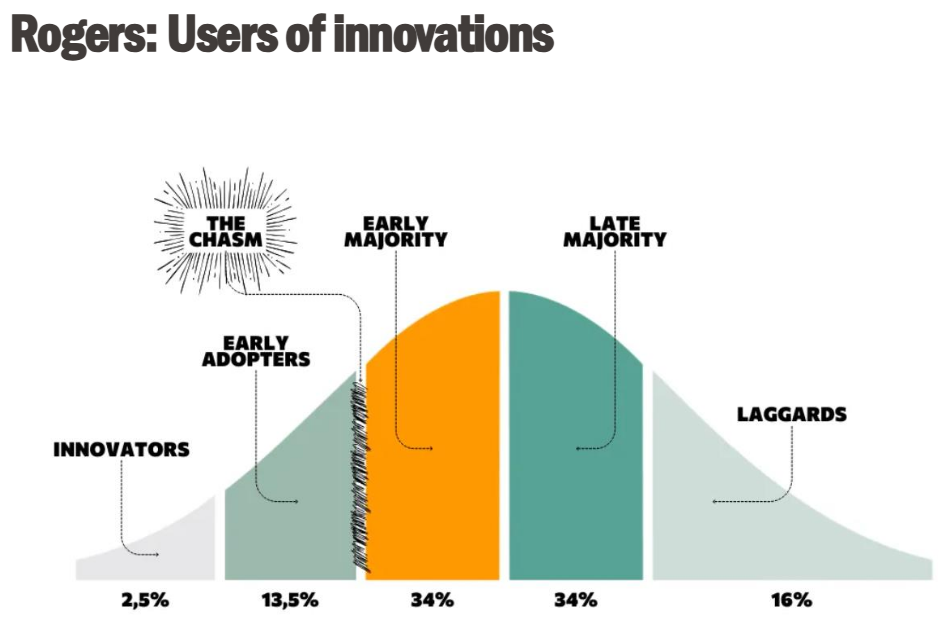
\includegraphics[width=0.5\linewidth]{IMAGES/NRJ_supply/Screenshot from 2025-04-30 08-56-36.png}
\end{figure}

Strategies to promote PV adoption : Focus on potential adopters first (collect low-hanging fruit), promote technology co-adoption (owners of electric vehicles and heat pumps are particularly keen on adopting PV), leverage social contagion (the presence of PV in personal networks positively influences).\\



\end{document}